% Paperformat
\documentclass[a4paper, 12pt]{scrartcl}
%\usepackage{cite}
\usepackage{ragged2e}
\usepackage{url}
\usepackage{bm} % bold math
\usepackage{nccmath} % medium fraction with mfrac 
\usepackage{amssymb}
\usepackage{graphicx}
\usepackage{amsthm} % theorems
\usepackage{hyperref}
\usepackage{float}
\usepackage{listings} % code
\usepackage{xcolor}
\usepackage{longtable} % breaks pages
\usepackage{tabularx}

\usepackage[style=alphabetic,backend=biber]{biblatex}
\addbibresource{bibtex.bib}

\definecolor{light-gray}{gray}{0.9}
\lstset{tabsize=2, linewidth=1.05\textwidth, framextopmargin=1em, basicstyle=\small\ttfamily}
\lstset{numbers=left,backgroundcolor=\color{light-gray}}
\newtheorem{theorem}{Theorem}[section]


\begin{document}
\def\myauthor{Martin Röbke} 
\def\mycoauthor{Dr. Johannes Fichte} 
\def\mytitle{Visualizing Dynamic Programming on Tree Decompositions} 
\def\mydate{\today} 
\def\mymatriculation{3949819}
\def\mybirthday{04.03.1995}
\def\myemail{Martin.Roebke@tu-dresden.de}

\begin{titlepage}
	\vspace*{\stretch{1}}
	\begin{center}
		\textsc{\large 
		{Technische Universität Dresden \\
			Fakultät Informatik} \\
		[8ex]}             
		{\Large\bfseries Bachelor Thesis}           \\[12ex]
		
		{\huge\bfseries \mytitle}                  \\[6.5ex]
		
		\vspace{12ex}
			
		
		{\Large 
		\begin{tabular}{p{0.4\textwidth}r}
		
			\textit{Author:}&  \textit{Supervisor:}\\
			
			\myauthor &  Dr. Johannes Fichte\\[20ex]
		
		\end{tabular}
		}
		
		
		\vfill
		\textsc{International Center For Computational Logic 		\\[4ex]}
		\mydate
	\end{center}
	\vspace{\stretch{2}}
\end{titlepage}
\newpage
%==============================================================================
%============== DECLARATION ===================================================
%==============================================================================
\section*{ }
\thispagestyle{empty}
{\huge\bfseries{Erklärung zur Urheberschaft}\vspace{20pt}}

\noindent
Hiermit versichere ich, dass diese Arbeit von mir persönlich verfasst ist und dass ich
keinerlei fremde Hilfe in Anspruch genommen habe. Ebenso versichere ich, dass diese Arbeit
oder Teile daraus weder von mir selbst noch von anderen als Leistungsnachweis oder als Leistung, die als Prüfungsvoraussetzung
zu erbringen war, andernorts bereits eingereicht wurden. Wörtliche oder sinngemäße Übernahmen aus anderen Schriften
oder Veröffentlichungen in gedruckter oder elektronischer Form sind gekennzeichnet.
Sämtliche Sekundärliteratur und sonstige Quellen sind nachgewiesen und in der Bibliographie aufgeführt.
Das Gleiche gilt für graphische Darstellungen und Bilder sowie für alle Internet-Quellen. \\[20pt]

\noindent
\myauthor \\
Matrikelnummer \mymatriculation\\
Geburtsdatum \mybirthday\\\\
TU Dresden E-Mail-Adresse:\\
 \myemail\\[40pt]


Dresden,  ............................. \hfill .............................
\begin{flushright}
	(Unterschrift)\hspace{1em}
\end{flushright}


\newpage

%==============================================================================
%============== ABSTRACT ======================================================
%==============================================================================
\section*{Abstract}
\vspace{4ex}

Answering questions that can be expressed using graph theory is increasingly interesting in scientific work.
Many problems such as Boolean satisfiability or problems related to traffic can be translated to and solved on a graph.
We think that utilizing the graph structure of problems and the connection between data points can help to improve algorithms concerning problems for different areas of interest.

The algorithms we visualize in this thesis use dynamic programming on tree decompositions of such graphs.
We preprocess the input graph into a customized tree-decomposition of small tree-width.
This gives us a description of the processing sequence for the algorithm, and allows 
with right hindsight for good parallelization and allows for faster solving times on larger instances.

To help for further refinement and visualization of the dynamic programming,
we specified a JSON-form to communicate between solvers and the newly created visualization tool \href{https://github.com/VaeterchenFrost/tdvisu}{TDVisu}.

As two reference implementations of dynamic programming on tree decompositions we selected the existing solvers \href{https://github.com/daajoe/GPUSAT}{GPUSAT} and \href{https://github.com/hmarkus/dp_on_dbs}{dpdb}.


\newpage

%  table
\tableofcontents

% chapter on next page
\newpage

%==============================================================================
%============== INTRODUCTION ==================================================
%==============================================================================

\section{Introduction}
Graphs are increasingly interesting in scientific work, as the applications of interconnected datasets grow.
Some use cases for example outlined \href{http://neo4j.com/use-cases}{here} do include fields of interest like
\begin{itemize}
	\item[-] Network and Database Infrastructure
	\item[-] Recommendation Engines
	\item[-] Artificial Intelligence and Analytics
\end{itemize}
It defines a \href{https://www.json.org/json-en.html}{JSON}-format specification for portability and customization of the visualization combined in one human-readable file and two reference implementations in actual solvers.
The implementation currently does not support hyper-graphs and assumes that each node in the tree decomposition has either one or two children.
The visualization output consists by default of scalable-vector-graphics \href{https://developer.mozilla.org/en-US/docs/Web/SVG}{SVG}, a very flexible text-based that can be compressed and modified very easily without loss of quality.
The images are split up into different views on the current state of the tree decomposition for consecutive user-defined time steps showing the progress of the dynamic programming.
As illustrations of the possibilities for an application smaller examples from the problem-types "\#SAT" and "minimal vertex cover" are presented,
as well as an example of a faulty tree-decomposition that occurred during development.
Intended audience: 
\begin{itemize}
	\item Developer of dynamic programming on tree decompositions for debugging.
	\item Researcher of such algorithms for comparisons and visualizations.
	\item Teachers or students looking for automatic visualization of their examples and the dynamic programming.
\end{itemize} 

The idea for this project comes from my supervisor Dr. Johannes Fichte, who works with many projects such as \href{https://github.com/hmarkus/dp_on_dbs}{dpdb} on solving monadic second order logic (MSOL\cite{Courcelle2012}) problems using highly parallelized architectures like graphics processing units or state of the art databases.
One early implementation is published in \cite{evaluationMSO} where for different real world examples the results looked promising
These projects are very competitive ????REF????? for solving even large instances of those problems.
The source code for TDVisu is available under GPL3 license.

\href{https://graphviz.org/}{Graphviz} is open source graph visualization software that provides
customizable visualization for directed and undirected graphs.
The information processed by graphviz 

intro. mit motivation und related work, state of the art, advancements.

Visualization Pipeline

Stand Umsetzung, Tools: Slack, Trello, GitHub, Presentations

%==============================================================================
%============== BACKGROUND ====================================================
%==============================================================================

\newpage
\section{Background}
\textit{This chapter provides the reader with a brief background for this work}.

We begin with a description on SAT and \#SAT as examples for a very general problem that can be described with monadic second order logic (MSOL).
Furthermore the general case of MSOL will be described, as well as the \textit{DIMACS}-file-format used in the projects.
The following section describes Tree Decompositions (TDs) which are the basis for our visualization. 
Finally we shortly discuss Courcelle's Theorem~\cite{Courcelle2012} as a related method of solving these problems.

\subsection{Boolean satisfiability problem}
\url{https://en.wikipedia.org/wiki/Boolean_satisfiability_problem}

SAT was the first known NP-complete problem, shown by Stephen Cook at the University of Toronto in 1971 \cite{SAT1971}

\begin{align*}
\text{literal}&\equiv \text{boolean variable v or its negation} \\
\text{clause}&\equiv \text{finite set of literals, interpreted as the disjunction} \\
\text{unit}&\equiv \text{clause with $|$c$|$=1} \\
\text{CNF formula}&\equiv \text{set of clauses, interpreted as their conjunction} \\
\text{var}&\equiv \text{set of variables contained in the clause or clause set C} \\
\text{assignment}&\equiv \text{$\alpha $:var(C) $\to $ \{0,1\}} \\
\text{satisfiedclause}&\equiv \text{if $\exists $v $\in $ var(c), v$\in $c and $\alpha $(v)=1 or $\neg $v$\in $c and $\alpha $(v)= 0. Otherwise falsified}\\ 
\text{satisfiedform}&\equiv \text{each clause in the formula is satisfied by assignment} \\
\end{align*}

Connection to graphs with \cite{DiplomarbeitZisser}

SAT Handbook:
Even finding a single solution can be a challenge
for such problems; counting the number of solutions is much harder.Not
surprisingly, the largest formulas we can solve for the model counting problem
with state - of - the - art model counters are orders of magnitude smaller than the
formulas we can solve with the best SAT solvers. Generally speaking, current
exact counting methods can tackle problems with a couple of hundred variables, while approximate counting methods push this to around 1, 000 variables.


\subsection{Monadic Second Order Logic}
See also figure~\ref{fig:logictheory}.

Explain graphs?Node, Edge

MSO graph properties are "fixed-parameter-tractable" with respect to clique-width and tree-width. 
\url{https://www.youtube.com/watch?v=hZI-wANHO1w} 5th workshop on Graph Classes, Optimization, and Width Parameters (GROW 2011)
2011-10-28.
MSO counting (k-colorings )and optimizing (distance between two vertices...) functions.
Interested in MSO logic over graphs.

Two types of MSO formulas \textit{or logical graph representations}.
\begin{itemize}
	\item MSO formulas
	\item MSO$_{2}$ formulas with edge quantification $\equiv$ MSO formulas over incidence graphs
\end{itemize}
\begin{itemize}
	\item G=(vertices, edges as binary relation)
	\item INC(G) = (vertices and edges, Inc)
		for G undirected: Inc(e,v) <-> v is a vertex of edge e
\end{itemize}
\begin{itemize}
	\item FPT for clique width
	\item FPT for tree-width
\end{itemize}
This can also be done for directed graphs!

Typical MSO$_{2}$ graph properties:

has a perfect matching
has a Hamiltonian circuit
spanning tree of degree $\le$ 3

The expressions have the form: "There exists a \textbf{set of edges} that is..." can not be transferred into "set of vertices"

\url{https://youtu.be/Wyn3djrYg7c?t=1385} Bruno Courcelle: Recognizable sets of graphs: algebraic and logical aspects 
\url{https://library.cirm-math.fr/Record.htm?idlist=2&record=19276851124910940339}
Recording during the thematic meeting: "Frontiers of reconnaissability" the April 29, 2014 at the Centre International de Rencontres Mathématiques (Marseille, France)

FPT for model checking:
An algorithm is FPT if it takes time $f(k)\cdot n^{c}$ for some fixed function f and constant c. The size of the input is n. 
The value k is a parameter of the input. 
This algorithm is then usable for small values of k. usually tree-width and clique width.


\subsection{DIMACS Format}
Developed in 1993 at Rutgers University.
DIMACS (the Center for Discrete Mathematics and Theoretical Computer Science)

Wolfram Language fully supports the DIMACS format for storing a single undirected graph.
\url{https://reference.wolfram.com/language/ref/format/DIMACS.html}

DIMACS CNF: This format is used to define a Boolean expression, written in conjunctive normal form.
\url{https://people.sc.fsu.edu/~jburkardt/data/cnf/cnf.html}

Other formats for WMC, different graphs...

Supported also in Maple \url{https://www.maplesoft.com/support/help/maple/view.aspx?path=Formats/CNF}

Examples in appendix

\subsection{Tree Decomposition}
\cite{DiplomarbeitZisser}chapter 2.2
Tree decompositions were originally introduced by Robertson and Seymour \cite{ROBERTSON198449} in 1984.
A \textit{tree decomposition} (TD) of a graph G is a pair $(T, \chi)$. $T$ is a tree and $\chi$ is a mapping which assigns each node $n~\in~V(T)$ 
a set $\chi(n) \subseteq V(G)$ called a \textit{bag}. Then $(T, \chi)$. $T$ is a TD if the following conditions hold:

\begin{itemize}
	\item[1.] for each vertex $v(n) \in V(G)$ there is a node $n \in V(T)$ such that $v \in \chi(n)$
	\item[2.] for each edge $(x,y) \in E(G)$ there is a node $n\in V(T)$ such that $x,y \in\chi(n)$
	\item[3.] if $x,y,z \in V(T)$ and $y$ lies on the path from x to z then $\chi(x) \cap \chi(z) \subseteq \chi(y)$.
\end{itemize}
The width $width(T)$ of a tree decomposition $T$ is $max_{n\in V(T)}(|\chi(n)|)-1$.
The tree width of a graph is the \textit{minimal width} over all tree decompositions of the graph.

!!!Example (can take one from the visualizations) also in \cite{pcgp2019} page 169
\subsection{Courcelle's Theorem}
\begin{quotation}
	Every graph property definable in monadic second-order logic (MSO) is decidable in linear time on graphs of bounded tree-width.\\
	{\small Courcelle, Bruno (1990)}\footnote{Courcelle, Bruno "The monadic second-order logic of graphs. I. Recognizable sets of finite graphs",\\ Information and Computation, 85 (1990) no. 1: 12-75}
\end{quotation}

For all $k \in \mathbb{N}$ and MSO-sentences F is the decision problem for a given graph G, whether $G \models F$ is true, in time $2^{p(tw(G))} \cdot |G|$ with a polynom p decidable.
\begin{itemize}
	
	\item \emph{drawback:} still expensive ($2^{p(tw G)}$, $2^{2^{(\#Q)}}$, large constants) \smallskip 

\end{itemize}

The workflow then looks like we see in figure~\ref{fig:UsageCourcelle}.

\begin{figure}[H]
	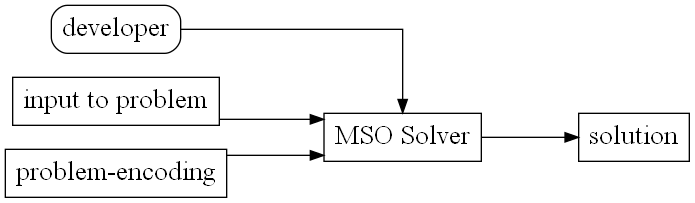
\includegraphics[height=0.2\textheight]{images/UsageCourcelle.gv.png}
	\caption{Implementation of the theorem}
	\label{fig:UsageCourcelle}
\end{figure}
%==============================================================================
%============== CONCEPT =======================================================
%==============================================================================
\newpage
\section{Concept}
We did setup a board with \url{https://trello.com} to track the progress and gather information connected to the project.
Discussion and problems were mostly discussed with a dedicated \href{slack channel}{https://slack.com/intl/en-de/} in the \emph{Collaborations Parameterized Algorithms and Complexity} team.

Research: language (python - explain) graph-construction (graphviz vs networkX), examples (diploma at first). 

My previous experience connected to this work mainly stemmed from these two very good courses:
\begin{itemize}
	\item Visualization with python from the lecture "Computational Physics" by Prof. Dr. A. Bäcker,
	chair of computational physics, TU Dresden 2016
	\item algorithms and various manipulations on graphs from the lecture "Graph Data Management and Analytics" by Hannes Voigt. \cite{VLGDMA}
\end{itemize}

%=========================== DOT Language ====================================

The nodes in the dot-language are \emph{labeled}, so creating a node takes one string identifier and
can additionally be provided a string label. Valid examples for IDs include: a, b, A1, node1.
The complete abstract grammar for DOT can be viewed at \href{https://graphviz.gitlab.io/_pages/doc/info/lang.html}{the DOT language}.

It supports directed (\textit{digraph} with edges indicated by '->') an undirected (\textit{graph} with edges indicated by '-{}-') graphs.
The visualizations presented here are constructed as undirected graphs, but would be easily extendable to directed representations since almost all operations keep the order of edge-endpoints given as input.

Another concept utilized were the sub-graphs and clusters available in DOT.
To get a well structured (bipartite) incidence graph, each partition is placed in an individual cluster
and sorted by node-label to easier find single nodes in potentially large clusters.


%==============================================================================
%============== PROJECT =======================================================
%==============================================================================
\newpage
\section{My Visualization Project}


Python because: Rich dependency environment. Fast prototyping. Simple tooling for debugging (pdb), static analysis (mypy), code-style (pylint, autopep8), packaging (pip, pypi).

Python 3.8 because: Python 3.8 was the newest python version at the beginning of the project, released on October 14th 2019. The change applied most times in this project would be \href{https://docs.python.org/3/whatsnew/3.8.html#f-strings-support-for-self-documenting-expressions-and-debugging}{f-string support} for shorter and easier to read string-building - for a longer list see \href{https://docs.python.org/3/whatsnew/3.8.html}{summary of release highlights}.

The development process was for most parts of the final software driven by evolutionary prototyping with the help of small and well understood examples such as \ref{fig:g41Digraph}. It helped to understand the possibilities of visualization in this domain and gather user input and requirements early \cite{rapidPrototypingOvermyer}. Some artifacts of the early prototypes with different graph-description languages can be still seen in the class \textit{Graphoutput} in \ref{chagraphoutput}.

The first steps were in \url{https://github.com/VaeterchenFrost/gpusat-VISU} and the first releases of the source code outsourced to\url{https://github.com/VaeterchenFrost/tdvisu}

The objective of this project was/is to support the visualization mainly to document and improve the development efforts of dynamic programming on tree decompositions.

The tree decompositions in every tested application were provided by the utility \url{https://github.com/mabseher/htd} (small but efficient C++ library for computing (customized) tree and hypertree decompositions).


% License

% Files / Classes / Methods

\subsection{Commandline and Configuration}


The \textit{tdvisu.visualization} expects the command line parameters in a format described by table~\ref{tab:optionstdvisu}.

\def\arraystretch{1.2}%  1 is the default
\begin{longtable}{|ll|}
	\caption{Usage visualization.py 
		\label{tab:optionstdvisu}}\\
	\hline 
	\multicolumn{2}{|c|}{[-h] [--version] [--loglevel LOGLEVEL] [infile] outfolder}
	\\[2ex]
	\endfirsthead

	infile=stdin &  Input file for the visualization must conform with the JsonAPI.md\\
	outfolder &  Foldername to output the visualization results to\\
	-{}-loglevel  &   set the minimal loglevel for the root logger\\
	-{}-version & show program's version number and exit\\
	-h, -{}-help & show the help message and exit\\
	\hline
\end{longtable}

We see that this input is very simple, and that the heavy lifting is done with the input file given in \textit{infile}.

One extra possibility for configuration comes with the method \textbf{logging\_cfg} from {tdvisu.utilities}. There are two example configurations provided with our project, one in the .yml, one in the .ini format. The implementation is very flexible in detecting which parser has to be applied - either via a dictionary-like or a configuration-like function. Both possibilities are documented in python's \href{https://docs.python.org/3/library/logging.config.html#logging-config-api}{logging configuration}.

Our default configuration in tdvisu/logging.yml and tdvisu/logging.ini provides one handler, two formatters and six loggers.

The \textbf{handler} is a stream handler to sys.stdout with level \textit{WARNING} and the the 'full'-formatter to format messages.

The \textbf{full-formatter} includes the full date and time up to milliseconds. After that we can expect the logging-level, filename and line where it was generated, and the message itself.

The \textbf{loggers} we use in our project are located in 
\begin{itemize}
	\item root, level: WARNING
	\item visualization.py, NOTSET
	\item svgjoin.py, NOTSET
    \item reader.py, NOTSET
	\item construct\_dpdb\_visu.py, NOTSET
	\item utilities.py, NOTSET
\end{itemize}
and can be individually customized using one configuration file.
With the command line parameter \textit{-{}-loglevel} we can modify the level of \textit{root} and it's associated handlers.

\subsection{Construct and Layout Solving Process}

After the configuration we instantiate a Visualization object as shown in listing~\ref{lst:visuinit} , which parses the VisualizationData with the help from our inspect\_json method. 

The main purpose of the initialization is parsing the input file containing visualization information.
This is encapsulated in \textit{read\_json}.

Next we want to extract information into two places: 
\begin{itemize}
	\item the instance variables 
	\begin{itemize}
		\item \textit{timeline}, describing the time steps on the tree decomposition
		\item \textit{tree\_dec}, describing the TD itself
		\item \textit{bagpre}, \textit{joinpre}, \textit{solpre} and \textit{soljoinpre} as names for different nodes in the produced visualization
	\end{itemize}
	\item \textit{VisualizationData} containing the data for 
	\begin{itemize}
		\item IncidenceGraphData in listing \ref{lst:incidencedata}
		\item GeneralGraphData in \ref{lst:gengraphdata}
		\item SvgJoinData in \ref{lst:svgjoindata}
		\item adjustable parameters affecting the visuals of the visualization
	\end{itemize}
\end{itemize}


\begin{lstlisting}[language={Python}, caption={Initializing a Visualization object}, label={lst:visuinit}]
def __init__(self, infile, outfolder) -> None:
	"""Copy needed fields from arguments and create VisualizationData.
	"""
	self.data: VisualizationData = self.inspect_json(infile)
	self.outfolder = outfolder
	
	self.tree_dec_digraph = None
	
def inspect_json(self, infile) -> VisualizationData:
	"""Read and preprocess the needed data from the infile into 
	VisualizationData.
	"""
	LOGGER.debug("Reading from: %s", infile)
	visudata = read_json(infile)
	LOGGER.debug("Found keys: %s", visudata.keys())
	
	try:
		_incid = visudata['incidenceGraph']
		_general_graph = visudata['generalGraph']
		_svg_join = visudata.get('svg_join', None)
		
		incid_data: IncidenceGraphData = None
		if _incid:
		_incid['edges'] = [[x['id'], x['list']]
		for x in _incid['edges']]
		incid_data = IncidenceGraphData(**_incid)
		visudata.pop('incidenceGraph')
		general_graph_data: GeneralGraphData = None
		if _general_graph:
		general_graph_data = GeneralGraphData(**_general_graph)
		visudata.pop('generalGraph')
		svg_join_data: SvgJoinData = None
		if _svg_join:
		svg_join_data = SvgJoinData(**_svg_join)
		if 'svg_join' in visudata:
		visudata.pop('svg_join')
		
		self.timeline = visudata['tdTimeline']
		visudata.pop('tdTimeline')
		self.tree_dec = visudata['treeDecJson']
		self.bagpre = self.tree_dec['bagpre']
		self.joinpre = self.tree_dec.get('joinpre', 'Join %d~%d')
		self.solpre = self.tree_dec.get('solpre', 'sol%d')
		self.soljoinpre = self.tree_dec.get('soljoinpre', 'solJoin%d~%d')
		visudata.pop('treeDecJson')
	except KeyError as err:
		raise KeyError(f"Key {err} not found in the input Json.")
	return VisualizationData(incidence_graph=incid_data,
													 general_graph=general_graph_data,
													 svg_join=svg_join_data,
													 **visudata)

\end{lstlisting}

\begin{lstlisting}[language={Python}, caption={SvgJoinData}, label={lst:svgjoindata}]
@dataclass
class SvgJoinData:
	"""Class holding different parameters to join the results."""
	base_names: Union[str, Iterable[str]]
	folder: Optional[str] = None
	outname: str = 'combined'
	suffix: str = '%d.svg'
	preserve_aspectratio: str = 'xMinYMin'
	num_images: int = 1
	padding: Union[int, Iterable[int]] = 0
	scale2: Union[float, Iterable[float]] = 1.0
	v_top: Union[None, float, str, 
	             Iterable[Union[None, float, str]]] = 'top'
	v_bottom: Union[None, float, str, 
	                Iterable[Union[None, float, str]]] = None	
\end{lstlisting}

\begin{lstlisting}[language={Python}, caption={IncidenceGraphData}, label={lst:incidencedata}]
@dataclass
class IncidenceGraphData:
	"""Class holding different parameters for the incidence graph."""
	edges: list
	subgraph_name_one: str = 'clauses'
	subgraph_name_two: str = 'variables'
	var_name_one: str = ''
	var_name_two: str = ''
	infer_primal: bool = False
	infer_dual: bool = False
	primal_file: str = 'PrimalGraphStep'
	inc_file: str = 'IncidenceGraphStep'
	dual_file: str = 'DualGraphStep'
	fontsize: int = 16
	penwidth: Union[float, str] = 2.2
	second_shape: str = 'diamond'
	column_distance: float = 0.5	
\end{lstlisting}

\begin{lstlisting}[language={Python}, caption={GeneralGraphData}, label={lst:gengraphdata}]
@dataclass
class GeneralGraphData:
	"""Class holding different parameters for the general graph."""
	edges: list
	extra_nodes: Optional[list] = None
	graph_name: str = 'graph'
	file_basename: str = 'graph'
	var_name: str = ''
	sort_nodes: bool = False
	need_adj_nodes: bool = False
	fontsize: int = 20
	first_color: str = 'yellow'
	first_style: str = 'filled'
	second_color: str = 'green'
	second_style: str = 'dotted,filled'
\end{lstlisting}

Next we call the method \textit{Visualization.tree\_dec\_timeline} that will start the visualization.
First it does a quick setup for a directed graph that 
\begin{itemize}
	\item is \textit{strict}, meaning a simple graph where equal edges are merged into one
	\item has an orientation where it grows with each "rank" of the nodes
	\item has a shape and a fill-color for it's nodes
	\item has a margin around it's bounding box.
\end{itemize}

Secondly it creates the basic bag-structure adding nodes and edges for all bags of the provided tree decomposition.

Now comes the heavy lifting when it iterates over the timeline, adding provided solutions and edges connecting those to the existing bags. We do this in two cycles, one two layout all nodes into their final position, and another one to create the final time-step images. A special case occurs when joining two solved bags into a new one.
In this case we basically remove old connections between the children and the parent node, insert the join-result into the graph and add connections from children to the join-result and from the join-result to the parent. Details for this function can be viewed in listing \ref{lst:forward-iterate}.
 
!!! Example !!!

The second run iterates backwards over all timesteps to hide later timesteps and emphasize the current node.
When rendering the graphs there is an added option to automatically \textit{view} the result (disabled by default. Details for this function can be viewed in listing \ref{lst:backward-iterate}.

\subsection{Create time steps for the underlying graph}
To get a more comprehensive insight into the solving process we decided to also highlight the parts of the 
graph that best describes the problem instance that the solver works on.

Because the information in the API does not directly include details about highlights in those graphs, we do construct this data on the fly.

First we select only bag ids from the timeline provided that present an IF-operation.
With additional data from \textit{IncidenceGraphData} we are able to reconstruct the
\begin{itemize}
	\item incidence graph,
	\item primal graph,
	\item dual graph
\end{itemize}
and with the edges from \textit{GeneralGraphData} we can construct a graph that should include the nodes we find in the bags of the TD.

% ----- Example for isolated nodes -------
Because graph representations of Boolean formulas are not necessarily connected ---EXAMPLE--- we make sure to include potentially isolated nodes into the graph.

\subsection{Incidence Graph}\label{sec:incid}
The incidence graph is a bipartite graph that we present in a way that creates a one to one correspondence with the 
Boolean formula it does represent. For an example of an incidence graph visualization see \ref{fig:incidencestep6}

This bipartite graph is prepared with good default values, but is customizable in many parameters.
Those values are:

\begin{enumerate}
	\item \textit{colors}, an iterable of colors that is used to color different nodes
	\item \textit{inc\_file}, basis for the file created that gets appended with the step number
	\item \textit{view}, could automatically open the generated files with the default program
	\item \textit{fontsize}, the size of all text in this graph
	\item \textit{penwidth}, width of the lines around nodes
	\item \textit{basefill}, filling of the background for nodes
	\item \textit{sndshape}, shape of the nodes with variables
	\item \textit{neg\_tail}, the shape of the edge-tail indicating a negated variable
	\item \textit{var\_name\_one(/two)}, prefix for nodes in the left (right) partition
	\item \textit{column\_distance}, the distance between both partitions
\end{enumerate}

We create the graph, add the necessary arguments and two sub-graphs. 
The first subgraph is called \textit{cluster\_clause} with it's label \textit{clauses}.
We add the clauses with their clause-ids starting at one sorted in ascending order from top to bottom.

The second sub-graph we call \textit{cluster\_ivar} labeled \textit{variables} gets all variables added to it, 
starting from variable-id one. 
This sub-graph does get the different provided \textit{colors} applied to its nodes and their adjacent edges.

The last step in this method is the highlighting of "active" parts in each time step beeing processed during it's dynamic programming. To accomplish this with as small overhead as possible, we apply and remove additional lines to the body of its graph source code. 
For highlighting there are two main cases:
\begin{itemize}
	\item There is no active clause in this step: we only reset highlighting
	\item Else: we also create new highlighting for clauses, variables and edges
\end{itemize}
In each case we create one image after the step to provide the inside generated.

\subsection{General Graph}
The so called "general graph" can represent the underlying graph for different problems, as well as primal and dual graph for Boolean formulas.
Because of its larger area of application the general graph was not as easy to layout as the incidence graph.
We did prepare two different layouts that should cover most cases and are toggled by the parameter \textit{do\_sort\_nodes}.
For smaller and dense graphs of up to 20 vertices it might be helpful to sort the nodes on a circle, while for larger or sparse graphs an organic layout may be more appropriate.

To layout these two options we chose the engine 
\begin{itemize}
	\item \textit{do\_sort\_nodes} true: circo (see \cite{ST99})
	\item \textit{do\_sort\_nodes} false: sfdp (see \cite{Hu05}) with the spring constant 'K' in virtual physical model set to 2.
\end{itemize}

Additional parameters used in both layouts are set to: not overlap nodes to easily identify each node, and draw the edges first. This should provide a minimally cluttered layout compared to the defaults, but could make edges ambiguous in some cases. Of course these layouts could use even more configuration than what was set for this version, a complete overview is provided in the \href{https://graphviz.org/doc/info/attrs.html}{graphviz-doc}. 

Only if the option to sort the nodes was chosen with \textit{do\_sort\_nodes} the method
\begin{enumerate}
	\item saves the current graph source 
	\item sets the layout engine to \textit{circo}
	\item adds edges between successive node-ids to form a closed circle
	\item runs the layout and reads back the output in plain dot-format
	\item reads the calculated positions for each node in the graph
	\item resets the source to step one, removing all temporary additions
	\item writes the calculated positions into each node
	\item sets the layout engine to an engine that uses those calculated positions later.
\end{enumerate}

We add the edges, and eventually the isolated nodes also, to the graph.
Then the highlighting for each time-step is done basically like in the incidence graph \ref{sec:incid}.
We allow one additional option that would depend on the concrete algorithm being visualized, and that is \textit{do\_adj\_nodes}.
In case the algorithm uses adjacent nodes they can be visualized with this flag using a third color.

% --- EXAMPLE
EXAMPLES

In each case we create one image after the time step to provide the inside generated.

\subsection{Joining SVG}{Joining each time step into one image}
Once all user defined images for one timeline are created, it would be nice to have only one file for each timestep
% perspective 

% Checking with www.deepcode.ai


\newpage
\section{Integration in GPUSAT}
To study and improve the handling of the C++ program was chronologically the first task I experimented with.
Getting the program up and running proved to be more difficult than we envisioned due to a probable bug in the driver when running OpenCL Drivers from CUDA on the Windows OS.

%=================Performance=======================
Impact on performance:
Utilizing small classes and \href{http://www.cplusplus.com/reference/sstream/stringstream/}{streams} we tried to keep the impact on performance during the solving process low. However running on the same thread especially for larger problem instances 

Some non-functional changes made to the source were 
\begin{itemize}
	\item[a)] some adjustments to satisfy the local compiler (shortening kernel string, replacing '\emph{and}' with '\&\&')
	\item[b)] some explicit casts
	\item[c)] fixed documentation of command line arguments
\end{itemize}

The functional changes were:
\begin{enumerate}
	\item allow tabs instead of spaces in input files
	\item output more information about the hardware used (device\_query)
	\item add verbose output globally toggled by a flag 
	\item decide on \url{https://en.wikipedia.org/wiki/DOT_\%28graph_description_language\%29} 
		as the intermediate format for storing graphs.
	\item start collecting information that might be needed for a visualization
		\emph{graphfile} for saving the decomposition graph
	\item add \emph{graphout }to solver flow to get automated insight into the structure of a run.
	
	\item add function \emph{solutiontable} to extract tables of variable assignments as a string
	\item add labels to each node (bags and solutions at this point)
	\item encapsulating the previous functions into gpusat::Graphoutput class and instantiate it in main.
	\item using the class functionality in the Solver
	\item changing enum to the \href{https://coders-corner.net/2017/08/13/scoped-vs-unscoped-enum/}{scoped enum class} for better encapsulation and strongly typed.
	\item with \href{https://github.com/daajoe/GPUSAT/commit/cfb310}{inlining gpusatutils} the current functionality of creating raw dot was completed.
	
	\item Experimented with Neo4j, but found the visualization in particular not that presentable. The functionality to create \href{https://neo4j.com/developer/cypher-resources/}{cypher-queries} for the SAT formula with primal, incidence and dual graph is still present in the class.
	\item The functionality to create the cypher-query for the graph of the tree-decomposition was added.
	\item Rename \textit{visualisierung} into \textit{visualization}
	\item Using \href{https://github.com/open-source-parsers/jsoncpp}{JsonCPP} for processing and formatting json objects in C++
	\item Setting format to {BasedOnStyle: LLVM, UseTab: Never, IndentWidth: 4, TabWidth: 4, ColumnLimit: 0}
	\item Creating a \emph{Grid} class for efficiently storing unsigned integer values in a two-dimensional structure
	based on ideas from \href{https://stackoverflow.com/questions/936687}{this thread}
	\item create \href{https://github.com/VaeterchenFrost/GPUSAT/blob/master/VisualCodeUsage.md}{guide} for remote development with \emph{Visual Code}
	\item Converted intermediate string operations to string-streams instead of files
	\item Updated README.md
	\item Added Doxygen for docbook, html, latex	
\end{enumerate}
Programm \url{https://github.com/VaeterchenFrost/GPUSAT} \\
Differences: \url{https://github.com/daajoe/GPUSAT/compare/master...VaeterchenFrost:master}  Commits 142 Files changed 94 
Nagoya talk:
Graphs for performance are Ordered by used time per algorithm - gpusat quite good

Working with cmake remotly. ssh @(sg1.)dbai.tuwien.ac.at
CPU branch wasn't working.
Only AMD/Nvidia graphics  with respective flags.

Manual configuration with the include options from \href{https://cmake.org/}{cmake} in \href{https://github.com/VaeterchenFrost/GPUSAT/blob/master/CMakeLists.txt}{CMakeLists.txt}
or with help from \url{https://marketplace.visualstudio.com/items?itemName=ms-vscode.cmake-tools}
to set up for the (potentially remote) environment.

\begin{itemize}
	\item 
	\item Options:
\end{itemize}


\begin{longtable}{ll}
	\caption{Usage: ./gpusat [OPTIONS]
		\label{tab:optionsgpusat}}\\
	\hline
	\vspace{0.5ex}
	\endfirsthead
-s, -{}-seed INT&  number used to initialize the pseudorandom number generator\\
	-f, -{}-formula TEXT &  path to the file containing the sat formula\\
	-d, -{}-decomposition TEXT  &   path to the file containing the tree decomposition\\
	-{}-CPU                   &    run the solver on a cpu\\
	-{}-NVIDIA                &    run the solver on an NVIDIA device\\
	-{}-AMD                   &    run the solver on an AMD device\\
	-{}-weighted              &   use weighted model count\\
	-{}-noExp                 &    don't use extended exponents\\
	-v, -{}-verbose            &    print additional program information\\
	-p, -{}-nopreprocess       &    skips the preprocessing step for debugging and visualization-purposes\\
	-w, -{}-combineWidth INT=20&    maximum width to combine bags of the decomposition\\
	-g, -{}-graph TEXT         &    filename for saving the decomposition graph\\
	-{}-visufile TEXT         &    filename for saving the visualization file\\

\end{longtable}
               
          


An example call with \textit{./gpusat -f ../examples/test\_da4\_1.cnf -v -p -d ../examples/td4p1.txt  -g ../examples/graphfileda41.txt -{}-visufile ../examples/visufileda41.json} enabled verbose output, disabled pre-processing to prevent the creation of bags with too many variables at once to be visualized, and creates full visualization output. 
The console output produced by this example call is listed in \ref{lst:outputGpusat}.




\subsubsection{Class Graphoutput}\label{chagraphoutput}
First steps to automatically visualize the tree decomposition of the solving process with its solutions.
Outputs a graph specified in gml\cite{Himsolt2010GMLAP} (Graph Modeling Language).
For our example for \#SAT~\ref{lst:g41digraphdot} with the bags and respective solutions as nodes connected to the bag they solve.

Two additional functions generate a \href{https://neo4j.com/docs/cypher-refcard/current/}{Neo4j Cypher} query with:
\begin{itemize}
	\item one graph representing the SAT formula and  queries to construct incidence, dual and primal representations.
	output as satFile = "cypherSatFormula.txt"
	\item one graph representing the tree decomposition of the primal graph with it's bags containing variables.
	output as tdFile = "cypherTreedec.txt"
\end{itemize}


\subsubsection{Class SolverVisualization}

To include the extraction of all necessary visualization information into the solver I created a separate fork.
To simplify the creation of valid json I selected the actively developed c++ library JsonCpp \url{https://github.com/open-source-parsers/jsoncpp} version 1.9.2 from the open-source-parsers repository.


\newpage
\section{Integration in dpdb}
The integration of the API with dpdb was easier to implement after the solving process instead of
hooking into the solving, 
provided that all necessary information got persisted in the database.
The integration is included in the TDVisu project as a separate python file.
A complete workflow can be accomplished using the arguments
\begin{itemize}
	\item -{}-store-formula as a problem specific option for Sat and SharpSat
	\item -{}-gr-file GR\_FILE for problems like VertexCover with graph input 
\end{itemize}
when calling dpdb.py\\
The integration for SharpSat was the first implemented in the file \textit{construct\_dpdb\_visu.py} with
the main parameters

\begin{itemize}
	\item
	\textbf{problemnumber}
	 the problem-id to select in the database
	 
	\item
	\textbf{-{}-twfile }TWFILE
	tw-file containing the edges of the graph 
	
	\item
	\textbf{-{}-outfile }OUTFILE
	 file to write the output to, default 'dbjson\%d.json'
	 
	\item
	\textbf{-{}-loglevel }LOGLEVEL
	 set the minimal loglevel for the root logger
	 
	\item
	\textbf{-{}-pretty}
	 pretty-print the JSON
	 
	\item
	\textbf{-{}-inter-nodes}
	Calculate and animate the shortest path between successive bags in the order of evaluation. To accomplish this task, an efficient implementation of the bidirectional Dijkstra's algorithm \cite{shortestPathAlgo} based on the implementation by NetworkX \cite{SciPyProceedings_11} in \href{https://networkx.github.io/documentation/networkx-2.1/reference/algorithms/generated/networkx.algorithms.shortest_paths.weighted.bidirectional_dijkstra.html#networkx.algorithms.shortest_paths.weighted.bidirectional_dijkstra}{bidirectional\_dijkstra}.
	in our case the weight function is always one, as the edges have no weight associated with them.
\end{itemize}
After the arguments are parsed by \href{https://docs.python.org/3/library/argparse.html}{pythons argparse} it is possible to adjust logging output by either providing a configuration file (\href{https://github.com/VaeterchenFrost/tdvisu/blob/master/tdvisu/logging.yml}{template} provided) or giving a minimal logging level per program argument.

!!! Database Config!!!

Next the \textit{create\_json}~\ref{lst:create-json} function connects to the database driver with 
the number of the stored problem. 
The "problem type" is available as a string in table \emph{public.problem}, and the appropriate class to prepare the json will be instantiated. At this time the solver handles the problems of \textit{satisfiability} (Sat), \textit{count solutions to a Boolean formula} (SharpSat) as well as \textit{minimum vertex cover} (VertexCover).


Beispiel

%==============================================================================
%============== APPLICATION ===================================================
%==============================================================================
\newpage
\section{Application and Images }

To collect the first parameters to be changed 

%==============================================================================
%============== SUMMARY =======================================================
%==============================================================================
\newpage
\section{Summary and Outline}
What is achieved?
What worked good, what bad?

%==============================================================================
%============== APPENDIX ======================================================
%==============================================================================
\newpage
\appendix
\section{Images}
\begin{figure}[H]
	\centering
	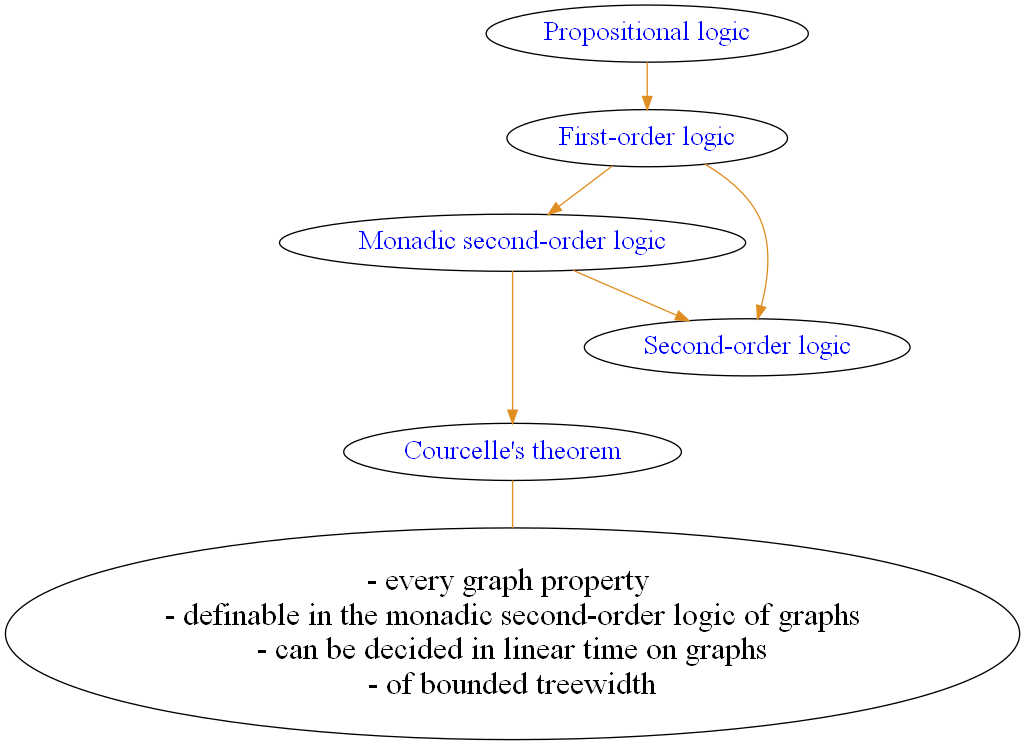
\includegraphics[width=0.8\linewidth]{images/logictheory.png}
	\caption{From propositional logic to monadic second order logic and Courcelle's Theorem}
	\label{fig:logictheory}
\end{figure}
\begin{figure}[H]
	\centering
	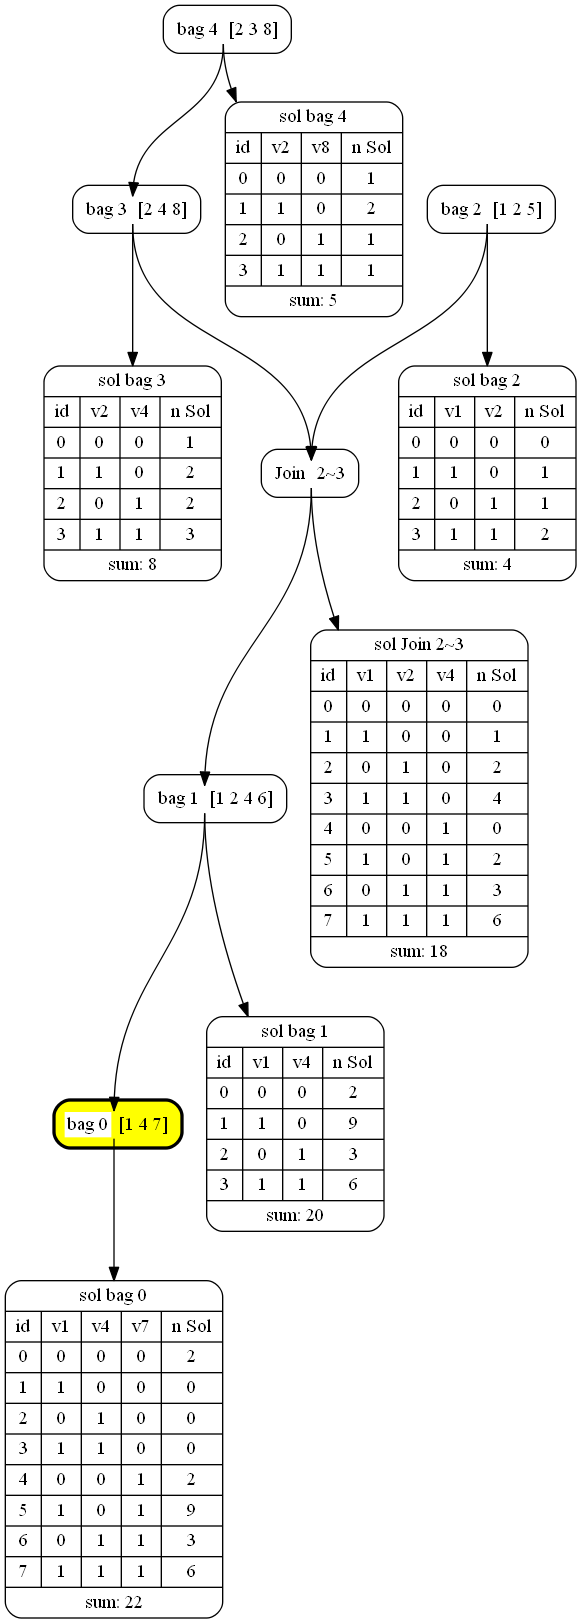
\includegraphics[height=\textheight]{images/g41digraphdot.png}
	\caption{Created scalable-vector-graphic directly from \ref{lst:g41digraphdot}}
	\label{fig:g41Digraph}
\end{figure}
\begin{figure}[H]
	\centering
	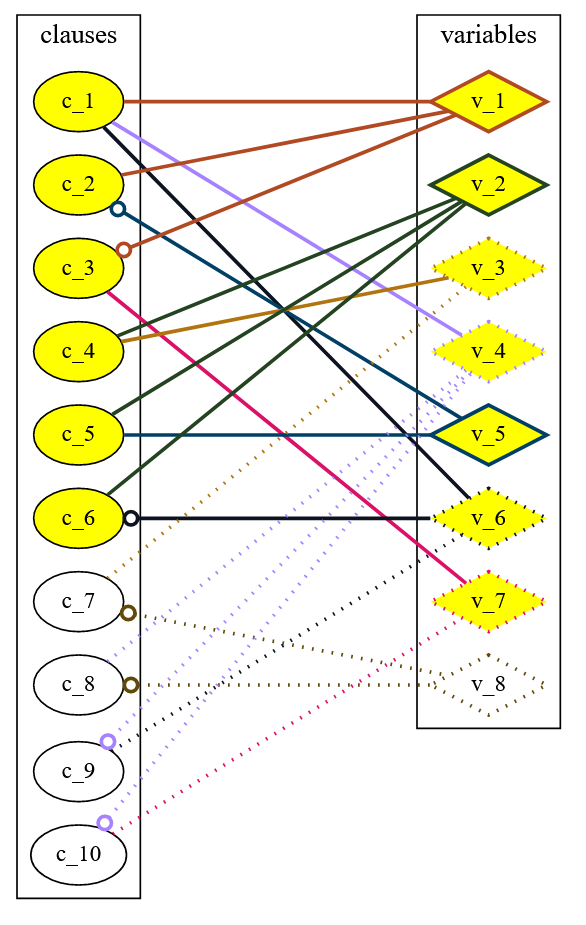
\includegraphics[width=0.4\linewidth]{images/IncidenceStep6.png}
	\caption{Example for an incidence graph from example 4.1}
	\label{fig:incidencestep6}
\end{figure}
\newpage
\section{Code Snippets}


\lstinputlisting[caption={The JSON format used to describe MSOL visualization on tree decompositions}, label={lst:jsonapi}]{includes/JsonAPI.txt}

\begin{lstlisting}[language={Python}, caption={Construct\_dpdb\_visu.py}, label={lst:create-json}]
def create_json(problem: int, tw_file=None, intermed_nodes=False):
	"""Create the JSON for the specified problem instance."""
	with connect() as connection:
		# get type of problem
		with connection.cursor() as cur:
			query = """SELECT name,type,num_bags 
			FROM public.problem WHERE id=%s"""
			cur.execute(query, (problem,))
			(name, ptype, num_bags) = cur.fetchone()
		
		constructor: IDpdbVisuConstruct  
		if ptype == 'SharpSat':
			constructor = DpdbSharpSatVisu(
						 connection, problem, intermed_nodes)
		elif ptype == 'VertexCover':
			constructor = DpdbMinVcVisu(
						 connection, problem, intermed_nodes, tw_file)
		return constructor.construct()
	return {} 
\end{lstlisting}

\begin{lstlisting}[language={Python}, caption={forward\_iterate\_tdg}, label={lst:forward-iterate}]
def forward_iterate_tdg(self, joinpre, solpre, soljoinpre) -> None:
"""Create the final positions of all nodes with solutions."""
	tdg = self.tree_dec_digraph                 # shorten name
	
	for i, node in enumerate(self.timeline):    # Create the positions
		if len(node) > 1:
			# solution to be displayed
			id_inv_bags = node[0]
			if isinstance(id_inv_bags, int):
				last_sol = solpre % id_inv_bags
				tdg.node(last_sol, solution_node(
				*(node[1])), shape='record')	
				tdg.edge(self.bagpre % id_inv_bags, last_sol)
			
			else:    # joined node with 2 bags
				suc = self.timeline[i + 1][0]   # get the joined bags
				
				LOGGER.debug('joining %s to %s ', node[0], suc)
				
				id_inv_bags = tuple(id_inv_bags)
				last_sol = soljoinpre % id_inv_bags
				tdg.node(last_sol, solution_node(
				*(node[1])), shape='record')
				
				tdg.edge(joinpre % id_inv_bags, last_sol)
				# edges
				for child in id_inv_bags:  # basically "remove" current
					tdg.edge(
							self.bagpre % child
							if isinstance(child, int) else joinpre % child,
							self.bagpre % suc
							if isinstance(suc, int) else joinpre % suc,
							style='invis',
							constraint='false')
					tdg.edge(self.bagpre % child if isinstance(child, int)
					         else joinpre % child,
					         joinpre % id_inv_bags)
				tdg.edge(joinpre % id_inv_bags, self.bagpre % suc
					if isinstance(suc, int) else joinpre % suc)
\end{lstlisting}

\begin{lstlisting}[language={Python}, caption={backwards\_iterate\_tdg}, label={lst:backward-iterate}]
def backwards_iterate_tdg(self, joinpre, solpre, soljoinpre,
                          view=False) -> None:
	"""Cut the single steps back and update emphasis acordingly."""
	tdg = self.tree_dec_digraph     # shorten name
	last_sol = ""
	
	for i, node in enumerate(reversed(self.timeline)):
		id_inv_bags = node[0]
		LOGGER.debug("%s: Reverse traversing on %s", i, id_inv_bags)
		
		if i > 0:
			# Delete previous emphasis
			prevhead = self.timeline[len(self.timeline) - i][0]
			bag = (
				self.bagpre %
				prevhead if isinstance(
				prevhead,
				int) else joinpre %
				tuple(prevhead))
			base_style(tdg, bag)
			if last_sol:
				style_hide_node(tdg, last_sol)
				style_hide_edge(tdg, bag, last_sol)
				last_sol = ""
		
		if len(node) > 1:
			# solution to be displayed
			if isinstance(id_inv_bags, int):
				last_sol = solpre % id_inv_bags
				emphasise_node(tdg, last_sol)
				tdg.edge(self.bagpre % id_inv_bags, last_sol)
			else:  # joined node with 2 bags
				id_inv_bags = tuple(id_inv_bags)
				last_sol = soljoinpre % id_inv_bags
				emphasise_node(tdg, last_sol)
			
		emphasise_node(tdg,
			self.bagpre %
			id_inv_bags if isinstance(id_inv_bags, int) else 
			joinpre % id_inv_bags)
		_filename = self.outfolder + self.data.td_file + '%d'
		tdg.render(
			view=view, format='svg', filename=_filename %
			(len(self.timeline) - i))

\end{lstlisting}

\section{Input Examples}

\lstset{numbers=none}
\begin{lstlisting}[caption={Edge encoding of example graph with 16 vertices}, label={lst:minvc16}]
p tw 16 36
1 2
2 1
2 3
3 2
3 4
4 3
3 5
5 3
4 5
5 4
4 6
6 4
6 7
7 6
7 8
8 7
8 9
9 8
9 10
10 9
9 11
11 9
11 12
12 11
12 13
13 12
12 14
14 12
11 14
14 11
14 7
7 14
6 15
15 6
15 16
16 15
\end{lstlisting}
\begin{lstlisting}[caption={CNF clauses from example 4.1 on page 27 \cite{DiplomarbeitZisser}}, label={lst:clausesDA41}]
p cnf 8 10
1 4 6 0
1 -5 0
-1 7 0
2 3 0
2 5 0
2 -6 0
3 -8 0
4 -8 0
-4 6 0
-4 7 0
\end{lstlisting}
\begin{lstlisting}[caption={CNF clauses from random example with 12 units},label={lst:example18-24}]
p cnf 18 24
-1 0
-2 0
-3 0
-4 0
-5 0
-6 0
-7 0
-8 0
-9 0
-10 0
-11 0
-12 0
-13 -14 -15 0
-13 -14 16 0
-13 -15 -16 -18 0
-13 -15 -17 0
13 14 16 -17 18 0
13 15 -16 -18 0
-14 -15 16 17 0
-14 15 -17 18 0
-14 15 17 -18 0
-15 -16 -17 18 0
15 -16 -17 -18 0
15 16 17 -18 0
\end{lstlisting}
\lstinputlisting[caption={DOT source for visualization of example 4.1}, label={lst:g41digraphdot}]{includes/g41digraphdot}
\lstinputlisting[caption={stdout of program gpusat with call \textit{./gpusat -f ../examples/test\_da4\_1.cnf -v -p -d ../examples/td4p1.txt  -g ../examples/graphfileda41.txt -{}-visufile ../examples/visufileda41.json}}, label={lst:outputGpusat}]{includes/outputGpusat.txt}

%==============================================================================
%============== BIBLIOGRAPHY ==================================================
%==============================================================================
\newpage
\printbibliography
%\bibliography{bibtex}{}
%\bibliographystyle{ieeetr}
\end{document}
